\chapter{Learning to identify clause types in Mandarin}
\label{chap:man-cl}

In this chapter, we will explore how Mandarin-acquiring children learn clause typing. As we have seen from last chapter, pragmatic information is crucial for finding the right clause type clustering. We find that a learner must have access to some pragmatic information in order to find the right clause types but this learner can succeed with very limited access to pragmatic information. 

As Mandarin [+int] and [imp] have different properties, would they be able to infer surface forms associated with these features from the input? Is pragmatics also crucial for Mandarin-acquiring children? How much pragmatics is required? In this chapter, I address these questions computationally, and found that surface morpho-syntactic features alone cannot help learners cluster sentences into the three clause types, and pragmatics is also needed. 

This chapter is organized as follows: we will review the properties of Mandarin [+int] and [imp], and children's knowledge regarding these properties. I then report results from a corpus study for Mandarin-speaking parents' input to children in  ~\ref{sec:mancl:corpus}. The data from the corpus study was used to simulate the two learners, \distlearner{} and \praglearner{}.  %

\section{Background}
\label{sec:mancl:bg}
\subsection{Clause types in Mandarin}
\label{sec:mancl:bg:theory}


In Mandarin, the [+int] value in $C^{0}$ does not trigger movements, but instead shows up in surface form as \twh-phrases, sentence final \tit{ma}, and A-not-A. For \twh-interrogatives, Mandarin \twh-phrases (\citealt{huang1982, cheng1991} among many others) do not need to be fronted to clause-initial position. Compare the declarative sentence in (\ref{bg-syn:dec-man}) with the \twh-interrogative in (\ref{bg-syn:wh-man}), the \twh-phrase \tit{shenme} occurs in the same position in the interrogative (\ref{bg-syn:wh-man}) as the noun phrase \tit{zaocan} in (\ref{bg-syn:dec-man}). 


%\begin{minipage}[t]{0.45\linewidth}	
\bex{bg-syn:dec-man}
\gll Xiaoxiao	chi-le zaocan.\\
Xiaoxiao eat-\Asp{} breakfast \\
``Xiaoxiao ate breakfast.''
\eex
\bex{bg-syn:wh-man}
\gll Xiaoxiao	chi-le \tun{shenme}.\\
Xiaoxiao eat-\Asp{} what \\
``What did Xiaoxiao eat?''
\eex


Interrogativity might also have effects on prosody. As mentioned before, \twh-phrases in Mandarin can be interrogative or indefinite (\ref{bg-syn:ambwh}), but interrogative \twh{} is normally associated with prosodic prominence (\cite{hu2002prosody, dong2009, yangyang2018} a.o.).

\bex{bg-syn:ambwh}
\gll Xiaoxiao	mei	chi	\tun{shenme}\\
Xiaoxiao	\Neg{}	eat	what\\
a.	What didn't Xiaoxiao eat?\\
b.	Xiaoxiao didn't eat anything.\\
\eex

\begin{figure}[H]
    \centering
    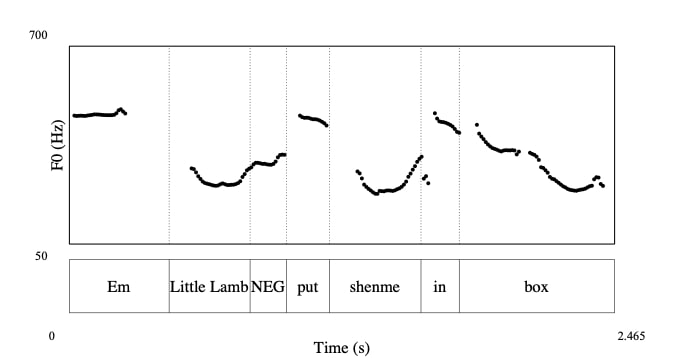
\includegraphics[width=0.6\textwidth]{figures/pitch-FC1wh.jpg}
    \caption{Pitch contour associated with a \twh-interrogative sentence}
    \label{fig:man:wh1}
\end{figure}

\begin{figure}[H]
    \centering
    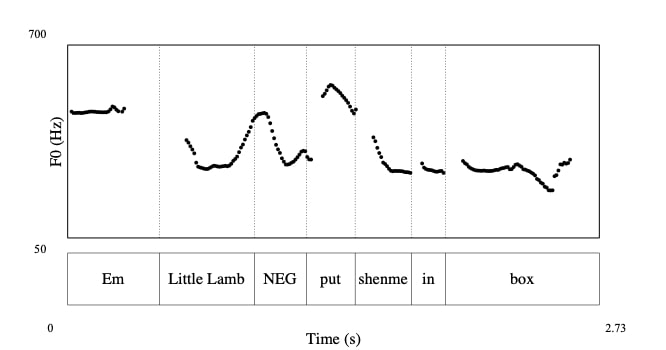
\includegraphics[width=0.6\textwidth]{figures/pitch-FC0wh.jpg}
    \caption{Pitch contour associated with a \twh-indefinite sentence}
    \label{fig:man:wh0}
\end{figure}

 Figure~\ref{fig:man:wh1} shows the pitch contour of the interrogative interpretation of \twh{} and Figure~\ref{fig:man:wh0} shows the indefinite interpretation. The former prosody is associated with [+int] and the latter with [$-$int], and the crucial difference is that the interrogative \tit{shenme} is produced with prosodic prominence (longer duration, extended lexical tone). 

Polar interrogatives in Mandarin also have SVO word order, but are distinguished from declaratives by surface features like the question-forming particle \tit{ma} or the A-not-A construction, as in (\ref{bg-syn:ma}) and (\ref{bg-syn:anota}).

\bex{bg-syn:ma}
\gll Xiaoxiao	chi-le	zaocan		\tun{ma}\\
Xiaoxiao	eat-ASP	breakfast	\Sfp{}\\
``Did Xiaoxiao eat breakfast?''
\eex
\bex{bg-syn:anota}
\gll Xiaoxiao	\tun{chi-mei-chi}	zaocan?\\
	Xiaoxiao	eat-\Neg-eat	breakfast\\
	``Did Xiaoxiao eat breakfast?''
\eex


Sentence final particles (SFPs) like \ma{} are  particles at the right edge of a clause (\citealt{chao1968, zhudexi, huang1982, cheng1991, liboya2006} among others). Many SFPs such as \tit{ba, ya} can occur in any clause type, but \ma{} can only occur in polar interrogatives that do not have the A-not-A form seen in (\ref{bg-syn:anota}). 

\begin{comment}
However, Mandarin learners have to contend with an additional difficulty, namely some of these phrases are not uniquely associated with interrogativity. Two prominent examples are \twh-phrases, which can have interrogative and non-interrogative interpretations in Mandarin, and the question particle \ma, which has a homophone that can occur in non-interrogative clauses.

\end{comment}


To summarize the discussion so far, the surface form of [+int] in Mandarin is sentence final particle \ma{}, A-not-A construction, \twh{} with prominence. 

Imperatives in Mandarin share many of the properties of imperatives in English, namely the lack of subjects. This clause type is sometimes marked by a negative modal \tit{bie} (and its etymologically related modal \tit{beng}), which only occurs in imperatives (\cite{chao1968, lithompson}):

\bex{ex:man:bie}
\bxl{ex:man:bie:imp}
\gll \tbf{Bie} pao!\\
Don't run\\
``Don't run!''
\ex 
\gll *Zhangsan \tbf{bie} pao.\\
Zhangsan don't run\\
(intended) Zhangsan doesn't run.
\exl
\eex 

Using \tit{bie} as a diagnostic for imperatives, we can see that Mandarin [imp] can be embedded (\cite{lithompson, chen2005imp}), and certain verbs like \tit{zhuzhang} selects [imp]:

\bex{ex:man:embed-imp}
\gll Wo \tun{zhuzhang} Lisi \tbf{bie} chu-guo.\\
I advocate Lisi don't exit-country\\
\trans ``I have the opinion that you don't leave the country.'' \hfill \textcite[p.458]{lithompson}
\eex

In sum, [+int] in Mandarin may show up in the surface form of the sentence as the presence of \twh{} with prominence, sentence final \tit{ma}, or A-not-A structure; [imp] shows as sentences without subjects or with second person subjects, and as special negative modal \tit{bie} or \tit{beng} in negative imperatives. 

Mandarin learner also face the same learning problem as English learners: the clause type feature is abstract and is related to a variety of surface forms, none of which is obligatorily present and many of which can occur in sentences with a different clause-type feature on $C^{0}$. For example, even though [imp] is related to null subjects, but since Mandarin is a pro-drop language, observing that a sentence does not have subjects does not necessarily mean that $C^{0}$ is [imp].  


\subsection{Mandarin-acquiring children's knowledge of clause types}
\label{sec:mancl:bg:child}
In this section we will look at evidence for Mandarin-acquiring children's knowledge regarding the features reviewed in the last section. For many of these features, we do not have a lot evidence from the comprehension side, and we have to rely on data from children's production alone to make inferences about their knowledge. As production might not be accurate reflection of children's grammar, we will be conservative in our inference.   

\tsc{\textpm subjects}  Children start producing sentences with subjects once they start producing two-word sentences. As Mandarin do not have subject-verb agreement, and do not have expletive subjects, it is hard to assess chidlren's knowledge regarding subjecthood. %However, studies have shown that when learning meanings of novel verbs, 
%However, studies show that as early as 17 months old, children could use whether nouns appear before or after a novel verb to infer whether the noun phrase is an agent 
%However, studies have shown that children could use canonical word order to infer meaning of novel verbs. Specifically, children are able to infer that nouns before the verb is normally the agent of an action (\cite{}).

\tsc{\textpm verbs} By 18 months old, Mandarin-acquiring infants demonstrate ability to categorize novel words as verbs using frequent frames related to verbs, such as auxiliaries and focus particles (\cite{zhangshili2015infant})
%Experimental results with 2-year-olds suggest that they associate the meaning of verbs with  \cite{lee2008manverb}
%verbs are produced at higher proportions than nouns in the early vocabulary of Chinese-speaking children, whereas the reverse pattern holds for their English-speaking coun- terparts (Tardif, 1996, in press; Tardif, Fletcher, Liang, & Zhang, 2002; Tardif, Gelman, & Xu, 1999). 

%and a large proportion of early verbs show signs of being treated as a coherent category (Xiao et al. 2006, Xiao 2006)
%experimental data on Mandarin-speaking children’s understanding of word order shows that they master this syntactic device at a very early stage (Li J. 2009).
\tsc{\textpm modal auxiliary}  \cite{zhangshili2015infant} find that 12mo use functional words to categorize content words, specifically they could use the negative imperative modal \tit{bie} to identify the follow-up item is a verb, suggesting that children might be sensitive to the presence of these modal auxiliaries.  %Children are found producing modal auxiliaries like \tit{neng} from 18 months old (\cite{}), but it is unclear whether 


\tsc{\textpm \tit{wh}-phrases} Children start producing interrogative \twh{} as early as 14 months old (\cite{lee1989acq, fan2012, linjing2014}); both comprhension experiments and corpus data show that they are also found to answer \tit{where}, \tit{who}, \tit{what} questions appropriately at 18 months old (\citealt{fan2012,moradlou2020}). While we have evidence that 3-year-olds can use prosodic prominence to infer whether the \twh-sentence is [+int] (\cite{WHanything}), we do not have evidence for younger children. In the corpus study, I follow the practice in the last chapter and classify \twh-phrases with focus particles and connectives (e.g. \tit{yaobu} ``if'') as `Unknown Functional Items' (UFI).

\tsc{A-not-A structure} As noted earlier, A-not-A structure and sentence-final \tit{ma} both distinguish interrogatives from declaratives in Mandarin. But while there are evidence suggesting that children start producing negation around 1.5 years old (\cite{lee1982,fan2007,li2019neg, huang2022manchild} among others), we do not have evidence for whether children perceive A-not-A sentences differently from simple negation sentences. Similarly, we do not have evidence for whether children treat \tit{ma} differently from sentences with other sentence final particles like \tit{ya}. I therefore simulated a conservative learner who do not have access to A-not-A and \tit{ma} features, and a knowledgeable learner who have access to these two features. 





\section{Corpus study}
\label{sec:mancl:corpus}

\subsection{Corpus and methods}
\label{sec:mancl:corpus:method}
This study used data from the Tong subcopora (\cite{TongCorpus}) from CHILDES (\cite{CHILDES}), which contains audio and video recordings of weekly hour-long free play sessions between Tong and his caregivers from 1;7-3;4 in Shenzhen, China where Mandarin is the language of the community. Although this corpus only contains data from one child, it is the most comparable to the Providence Corpus in the child’s age range and availability of audio/video data. If more corpora from Mandarin-speaking children become available in the future, the methodology developed here can be applied to them. Another problem with the corpus is that it does not have data from before when the child is 18 months old, which is older than our assumed age that children figure out the clause type categories and older than the children in the English corpus study. However, while the pragmatics of parent-child interaction might change with children's age, the morpho-syntactic properties of parents' sentences should stay constant. Therefore, we assumed that the input sentences share similar properties as parents' sentences before Tong turns 18 months old. Once the corpus releases data from before 18 months old, we would apply the same methodology to these data. 

We sampled 500 conversational turns from each session from when the child was 01;07;18 to 2;2;16. Each session was coded by two annotators independently for the Clause Type and Speech Act information (mean cohen's $\kappa$: 0.8). For the morpho-syntactic features, initial annotation was generated by a script (\textcolor{red}{url}) using the morphological tagging provided by the corpus, and then manually corrected. In total, 4501 utterances were annotated. 

\subsubsection{Clause Type}

Same as the English corpus study reported in the last chapter, each sentence was annotated with their clause type category, \diis{} (\ref{ex:mancl:annt:cl:dec}-\ref{ex:mancl:annt:cl:imp}). Sentences with only one noun phrase or injectives were annotated as ``fragments'':\footnote{Sentences without verbs might not be fragments in Mandarin, as the copula \tit{shi} ``be'' is optional:
\begin{xlist}
\ex 
\gll Zhe wode.\\
This mine.\\
\trans `This is mine.'
\end{xlist}
}

\bex{ex:mancl:annt:cl}
\bxl \label{ex:mancl:annt:cl:dec}
\gll Wazi shi le.\\
Sock wet \Sfp{}\\
``Your socks got wet.'' \hfill Declarative
\ex \label{ex:mancl:annt:cl:int}
\gll Kandao le ma?\\
See \Asp{} \Sfp{}\\
\trans``Do you see it?''  \hfill Interrogative
\ex \label{ex:mancl:annt:cl:imp}
\gll Gei wo hongse de na-ge.\\
Give me red \tsc{poss} that-\Cl{}\\
\trans``Give me the red one.'' \hfill Imperative
\ex \label{ex:mancl:annt:cl:frag}
\gll Ai-ya!\\
\tsc{intj} \\
\trans ``Wow!'' \hfill Fragments
\exl
\eex

The three major speech acts were also annotated, same as English.

\subsubsection{Morpho-syntactic features for clause typing}

As reviewed in the last section, Mandarin-acquiring children at 18 months old can perceive many morpho-syntactic properties related to clause typing in Table~\ref{tab:mancl:grammar}. In particular, they might be able to identify the subject, verb, auxiliary of the sentence, and distinguish functional from lexical items. We additionally adopted the conservative assumption that children at this age might not be able to identify all the \twh-items at this stage,but they might be able to classify them as functional elements, as they may know the distinction between functional and content elements. We therefore put \twh-items, quantifiers, connectives (e.g. \tit{haishi}, the interrogative ``or''), and focus particles in one category ``unknown functional item (UFI),'' and annotated its position in a sentence: sentence initial, sentence-medial but before the verb, after the verb, or sentence final. In addition to these surface features that were also annotated in the English corpus study, we also annotated for whether the sentence contains an A-not-A structure, and whether there is a sentence-final \tit{ma} particle. But since we do not have evidence for whether children around 18 months can perceive these two cues, as discussed in the last section, when simulating children's learning process, we will compare conservative models without these two cues, and knowledgeable models with these two cues.


Each sentence was annotated with whether or not a surface feature is present. Table~\ref{tab:mancl:formal-schema} summarizes the surface features we annotated and their examples.  


\begin{exe} \label{mancl:schema:formal:verb}
\ex 
\gll \tbf{kan} zhe-ge.\\
Look this-\Cl{}\\
\trans `Look at this one!'' \hfill +Verb
\end{exe}

\bex{mancl:schema:formal:subj}
\gll \tbf{Wo} zhidao.\\
I know\\
\trans ``I know.'' \hfill +Subject
\eex

\begin{comment}
\bex{mancl:schema:formal:asp}
\bxl
\gll Mama mei gei ni mai \tbf{guo} zhege wanju\\
Mom \Neg{} to you buy \Asp{} this toy\\
\trans`` Mom never bought this toy for you.'' \hfill +Aspect
\exl
\eex
\end{comment}

\bex{mancl:schema:formal:aux}
\bxl
\gll Xiaopengyou bu-\tbf{neng} peng.\\
Children \Neg-can touch\\
\trans ``Children can't touch (this).'' \hfill +Auxiliary
\exl
\eex

\bex{mancl:schema:formal:ufi}
+ Unknown functional items:
\bxl
\gll \tbf{Yaobu} na zhe-ge kapian lai jiao ba\\
%要 不 拿 这 个 卡片 来 教 吧 .
What-if take this-\Cl{} card to teach \Sfp{}\\
\trans ``What if (you) teach with this card.''  \hfill Sentence-initial UFI

\ex
\gll Zheli \tbf{hai} you labi.\\
Here also have crayon\\
\trans ``There's also crayons." \hfill Pre-verbal UFI
\ex
\gll  Limian you \tbf{shenme} ya?\\
Inside have what \Sfp{}\\
\trans ``What's inside?" \hfill Post-verbal UFI
\ex 
\gll Guolai \tbf{ba}\\
Come \Sfp{}\\
\trans ``Come here!'' \hfill Sentence final particle
\exl
\eex

\bex{mancl:schema:formal:anota}
+ A-not-A: 
\bxl
\gll Jintian \tbf{leng-bu-leng} a?\\
Today cold-\Neg-cold \Sfp{}\\
\trans ``Is it cold today?" \hfill \tit{Adj-not-Adj}
\ex 
\gll Ni \tbf{hui-bu-hui} xiezi?\\
You can-\Neg-can write\\
\trans ``Can you write? \hfill \tit{Aux-not-Aux}
\ex \gll Ni \tbf{you-mei-you} xiaoqiche?\\
You have-\Neg-have car\\
\trans ``Do you have cars?'' \hfill \tit{V-not-V}
\ex 
\gll \tbf{Chuan-hao} yifu \tbf{meiyou}?\\
Put-well cloth \Neg{}\\
\trans ``Did you put on your coat?'' \hfill \tit{A-not}
\exl
\eex

\bex{mancl:schema:formal:ma}
\gll Xiayu le \tbf{ma}?\\
Rain \Asp{} \tsc{ma}\\
\trans ``Is it raining?'' \hfill +\tit{ma}
\eex

\subsection{Results}
\label{sec:mancl:corpus:results}

\subsubsection{Overview}
\label{sec:mancl:corpus:results:mapping}

In total, 3077 utterances were annotated. Figure~\ref{fig:man-real-cldist} shows the distribution of clause types in the dataset. Same as results in the English dataset, Declarative clauses are the most frequent clause type, followed by interrogatives and imperatives. 

\begin{figure}[H]
    \centering
    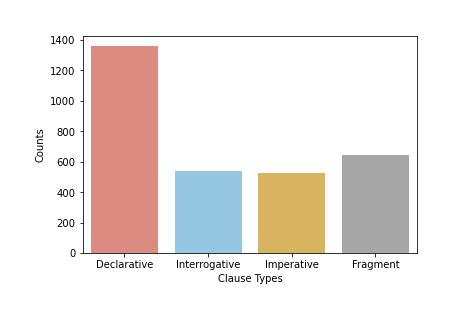
\includegraphics[width=0.7\textwidth]{figures/man-real-cldist.jpg}
    \caption{Distribution of clause types in the corpus}
    \label{fig:man:real-cldist}
\end{figure}

Within interrogatives (Figure~\ref{fig:man:real-subint}), \twh-interrogatives are more frequent, a pattern similar to English; followed by A-not-A and \tit{ma}-interrogatives. Disjunctive interrogatives with \tit{haishi} ``or'' are relatively rare. 
\begin{figure}[H]
    \centering
    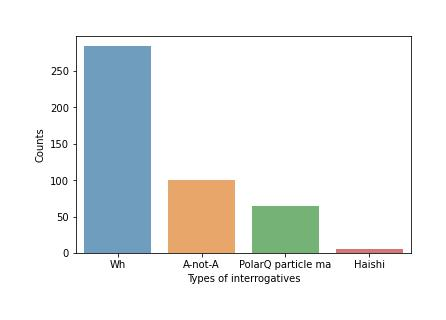
\includegraphics[width=0.7\textwidth]{figures/man-real-subint.jpg}
    \caption{Subcategories of interrogatives}
    \label{fig:man:real-subint}
\end{figure}

\bex{ex:man:int:corpus}
\bxl\label{ex:man:int:wh}
\gll Zhe \tit{shenme}?\\

\ex\label{ex:man:int:anota}
\ex\label{ex:man:int:ma}
\ex\label{ex:man:int:haishi}
\exl
\eex

\begin{figure}[H]
    \centering
    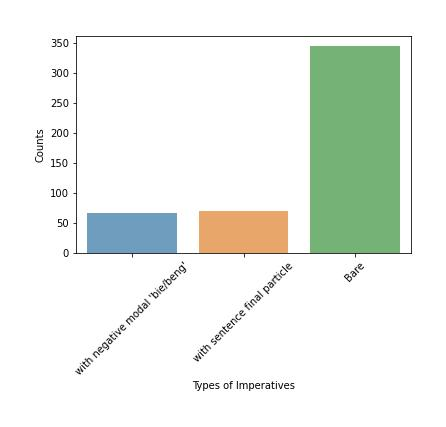
\includegraphics[width=0.7\textwidth]{figures/man-real-subimp.jpg}
    \caption{Subcategories of imperatives}
    \label{fig:man:real-subimp}
\end{figure}

Imperatives (Figure~\ref{fig:man:real-subimp}) sentences mostly come without any marker like (\ref{ex:man:impbare}); \tit{bie}-imperatives and SFP-imperatives are equally frequent. 


\bex{ex:man:imp:corpus}
\bxl\label{ex:man:impbare}
\gll Kan zhege shi shenme dongxi\\
look this is what thing\\
``See what this is!''  \hfill
Mother of Tong, Session 02;00;19\\
Imperative (used as a question)

\ex \label{ex:man:impbie}
\gll \tbf{Bie} fan le!\\
Don't turn \Asp{}\\
``Stop messing around!'' \hfill Mother of Tong, Session 02;00;09\\
\tit{Bie}-imperative
\ex \label{ex:man:impba}
\gll Reng zheli \tbf{ba}\\
throw here \Sfp{}\\
\trans ``Throw it here!''
\hfill Mother of Tong, Session 02,01,17\\
SFP imperative
\exl
\eex

\begin{figure}[H]
    \centering
    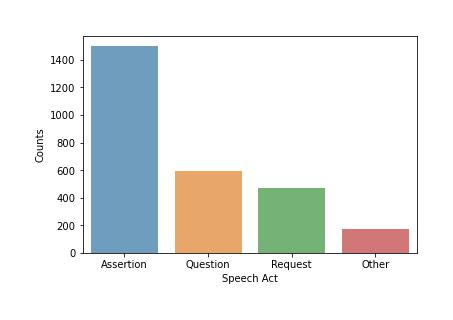
\includegraphics[width=0.7\textwidth]{figures/man-real-sp.jpg}
    \caption{Distribution of speech acts in the corpus}
    \label{fig:man-real-sp}
\end{figure}

\begin{figure}[H]
    \centering
    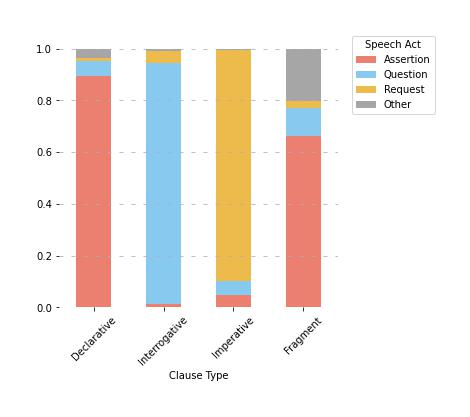
\includegraphics[width=0.7\textwidth]{figures/man-real-clsp.jpg}
    \caption{The speech acts performed by each clause type in parents' speech}
    \label{fig:man-real-clsp}
\end{figure}

\begin{figure}[H]
    \centering
    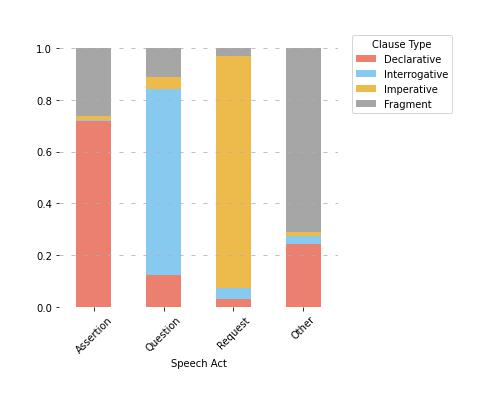
\includegraphics[width=0.7\textwidth]{figures/man-real-spcl.jpg}
    \caption{The clause type used to express each speech act in parents' speech}
    \label{fig:man-real-spcl}
\end{figure}

\subsubsection{Morpho-syntactic cues}
\label{sec:mancl:corpus:results:syn}


\begin{figure}[H]
    \centering
    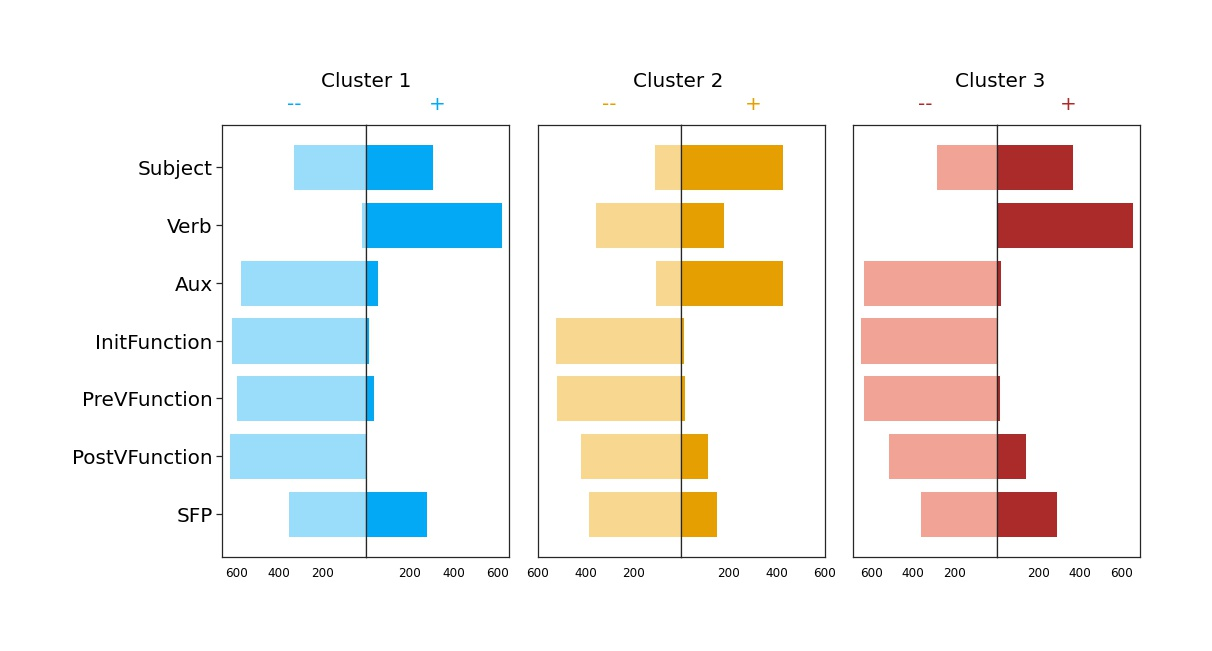
\includegraphics[width=1\textwidth]{figures/man-baseline-conservative-syncluster.jpg}
    \caption{Number of sentences with/without various formal cues in each clause type; darker colors represent number of sentences with the cue, lighter colors, number of sentences without the cue }
    \label{fig:man-real-syncluster}
\end{figure}


%\subsubsection{Informativeness of the cues}
%\label{sec:mancl:corpus:results:supervised}


\section{Modeling the learning of clause type in 
Mandarin}
\label{sec:mancl:model}


\subsection{Performance of the \dlearnerabbr{} model}
\label{sec:mancl:model:results:d}

Figure~\ref{fig:man-baseline-heatmap} shows the proportion of \diis{} in each identified cluster, and Figure~\ref{fig:man-baseline-heatrev} shows the proportion of sentences clustered together. In other words, Figure~\ref{fig:man-baseline-heatmap} shows whether each cluster mostly consists of one clause type, and Figure~\ref{fig:man-baseline-heatrev} shows whether each clause type is put in one cluster.  



\begin{figure}[H]
    \centering
    \includegraphics[width=0.7\textwidth]{figures/man-baseline-conversative-heat.jpg}
    \caption{The proportion of \diis{} in each of the three clusters identified by the \dlearnerabbr{} model}
    \label{fig:man-baseline-conversative-heat}
\end{figure}


\begin{figure}[H]
    \centering
    \includegraphics[width=0.7\textwidth]{figures/man-baseline-conversative-heatrev.jpg}
    \caption{The proportion of actual \diis{} clustered in one category}
    \label{fig:man-baseline-conversative-heatrev}
\end{figure}

\begin{figure}[H]
    \centering
    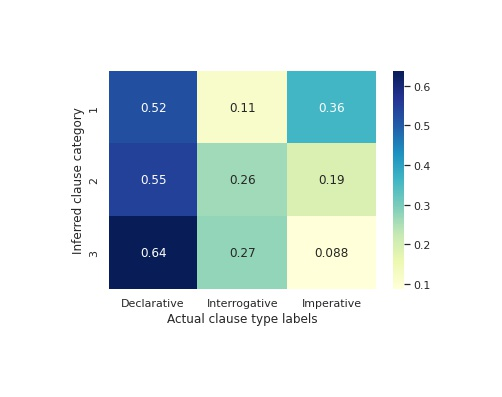
\includegraphics[width=0.7\textwidth]{figures/man-baseline-mid-heat.jpg}
    \caption{The proportion of \diis{} in each of the three clusters identified by the \dlearnerabbr{} model}
    \label{fig:man-baseline-mid-heat}
\end{figure}


\begin{figure}[H]
    \centering
    \includegraphics[width=0.7\textwidth]{figures/man-baseline-conversative-heatrev.jpg}
    \caption{The proportion of actual \diis{} clustered in one category}
    \label{fig:man-baseline-mid-heatrev}
\end{figure}

Overall, Figure~\ref{fig:man-baseline-heatmap} shows that the \dlearnerabbr{} model identifies an interrogative cluster and a declarative cluster. Cluster~$0$ mostly contains interrogative clauses, as 90\% of sentences in this cluster are interrogative; Cluster~$2$ is mostly declarative, and 86\% of the data in this cluster are declaratives. Cluster~$1$ is split between declaratives and imperatives. Figure~\ref{fig:baseline-heatrev} shows that 87\% of interrogatives and 93\% of imperatives are clustered together in Cluster~$0$ and $1$ respectively. While most of declaratives are classified in Cluster~$2$, a proportion is classified in Cluster~$1$.

These results seem to suggest that the \dlearnerabbr{} found two out of three clause types, but how do these clause types look like? Did the model find the right morpho-syntactic properties to associate with each clause type? Figure~\ref{fig:baseline-syncluster} plots the morpho-syntactic profile of each cluster identified by the \dlearnerabbr{}. Darker colors represent sentences with the morpho-syntactic property, and lighter colors represent sentences without the property. 

\begin{figure}[H]
    \centering
    \includegraphics[width=1\textwidth]{figures/man-baseline-syncluster.jpg}
    \caption{The number of sentences with/without certain formal features in each cluster (Cluster 0 $\sim$ Interrogatives, Cluster 1 $\sim$ Imperatives, Cluster 2 $\sim$ Declaratives), darker colors represent the number of sentences with the feature. UFI stands for Unknown Functional Item (e.g. \twh{}), see Table~\ref{tab:mancl:formal-schema} for details.}
    \label{fig:man-baseline-syncluster}
\end{figure}

We can see that Cluster~$0$, which is 90\% interrogative clauses, is associated with [+int] morpho-syntactic properties such as subject-auxiliary inversion and sentence-initial unknown functional item (e.g. \twh{}).

\subsection{Performance of the \plearnerabbr{} model}
\label{sec:mancl:model:results:d}

Figure~\ref{fig:man-target-heatmap} shows the proportion of \diis{} in each identified cluster, and Figure~\ref{fig:man-target-heatrev} shows the proportion of sentences clustered together. 
\begin{figure}[H]
    \centering
    \includegraphics[width=0.7\textwidth]{figures/man-target-heatmap.jpg}
    \caption{The proportion of \diis{} in each of the three clusters identified by the \plearnerabbr{} model}
    \label{fig:man-target-heatmap}
\end{figure}




\begin{figure}[H]
    \centering
    \includegraphics[width=0.7\textwidth]{figures/man-target-heatrev.jpg}
    \caption{The proportion of actual \diis{} clustered in one category}
    \label{fig:man-target-heatrev}
\end{figure}
%Rand comparison

%confusion matrix

We can see that the \plearnerabbr{} model clearly identifies a declarative, an interrogative, and an imperative cluster: 94\% of Cluster~$0$ are interrogatives, 86\% of Cluster~$1$ are declaratives, and 70\% of Cluster~$2$ are imperatives. The three clause types in English are also mostly clustered together by the model: 95\% of declaratives, 90\% of interrogatives, and 87\% of imperatives are clustered together in Cluster~$1$, $0$, $2$ respectively. Compare to \dlearnerabbr{}, this learner is able to find the right clause types in English.


Figure~\ref{fig:man-target-syncluster} shows the morpho-syntactic profile of each cluster identified by the \plearnerabbr{}. 

\begin{figure}[H]
    \centering
    \includegraphics[width=1\textwidth]{figures/man-target-syncluster.jpg}
    \caption{The number of sentences with/without a formal property in each cluster (Cluster 0 $\sim$ Interrogatives, Cluster 1 $\sim$ Declaratives, Cluster 2 $\sim$ Imperatives), darker colors represent the number of sentences with the property, lighter colors represent sentences without the property.}
    \label{fig:man-target-syncluster}
\end{figure}

The profile of the three clusters resembles the profile of \diis{} in our corpus study (Figure~\ref{fig:man-real-syncluster}). The cluster for interrogatives has more sentences with subject-auxiliary inversion and clause-initial unknown functional items (e.g. \twh{}), and the cluster for imperatives is characterized by the lack of subjects and verb suffixes. 

\subsection{Simulations with noisy pragmatic information}
\label{sec:mancl:model:results:noisy}

Figure~\ref{fig:noisy-rand-compare} shows the simulations with 0-100\% noise. The performance of the \dlearnerabbr{} model in our last simulation is marked by the dotted line. As can be seen, the \plearnerabbr{} learner outperforms the \dlearnerabbr{} learner up until there is around 80\% of noise in speech act, and even at 80\% level there are iterations that outperforms the \dlearnerabbr{}. This suggests that a little pragmatics goes a long way, as the learners with noisy pragmatic information still outperforms the one without. 

\begin{figure}[H]
    \centering
    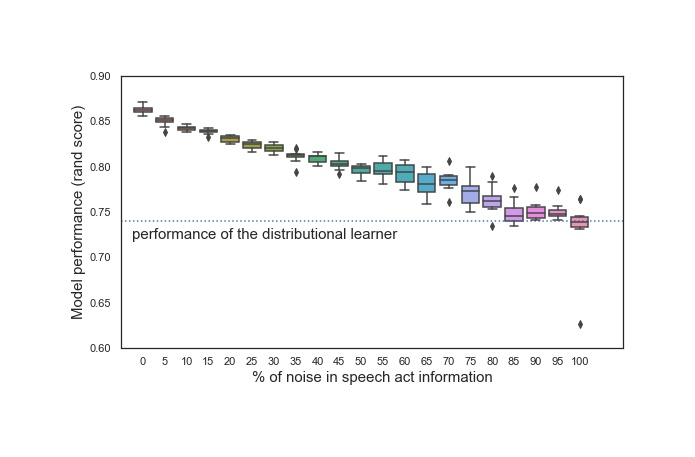
\includegraphics[width=1\textwidth]{figures/noisy-rand-compare.jpg}
    \caption{Performance of the \plearnerabbr{} model with different levels of noise in the speech act information; dotted marks the rand score of the \dlearnerabbr{} learner}
    \label{fig:noisy-rand-compare}
\end{figure}


Looking at the learner at maximum noise level, we can see that the \plearnerabbr{} reverts back to the performance of the \dlearnerabbr{} fails to identify a cluster for declaratives (Figutre~\ref{fig:noisy100-heatmap}. Similar to the distributional learner, the cluster for imperatives also have declaratives (\ref{fig:noisy100-heatrev}). 



\begin{figure}[H]
    \centering
    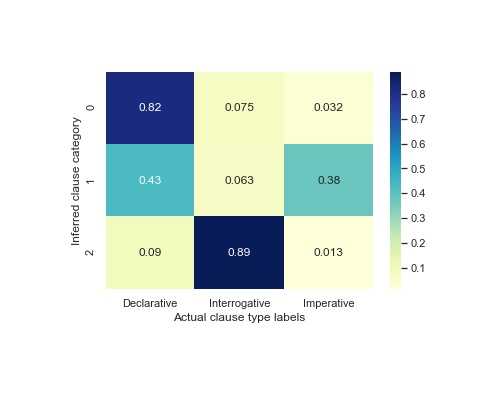
\includegraphics[width=0.7\textwidth]{figures/noisy100-heatmap.jpg}
    \caption{The proportion of \diis{} in each of the three clusters (100\% noise in speech act information) }
    \label{fig:noisy100-heatmap}
\end{figure}

\begin{figure}[H]
    \centering
    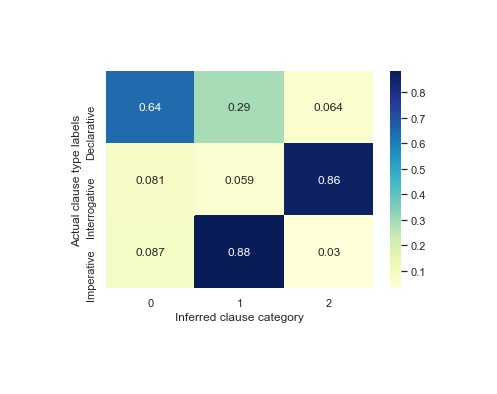
\includegraphics[width=0.7\textwidth]{figures/noisy100-heatrev.jpg}
    \caption{The proportion of actual \diis{} clustered in one category}
    \label{fig:noisy100-heatrev}
\end{figure}

Looking at the morpho-syntactic profile of this model with random speech act information behaves like the \dlearnerabbr{} model, and fails to identify the properties of English imperatives and declaratives.

\begin{figure}[H]
    \centering
    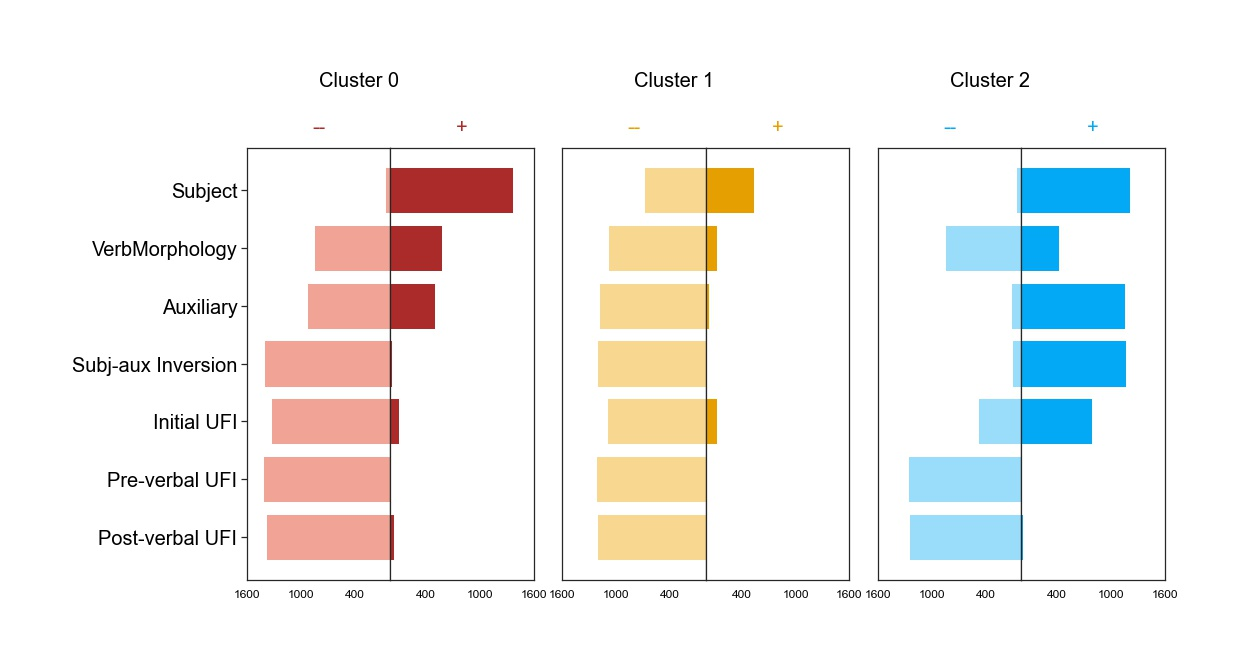
\includegraphics[width=1\textwidth]{figures/noisy100-syncluster.jpg}
    \caption{The number of sentences with/without certain formal features in each cluster (Cluster 0 $\sim$ Interrogatives, Cluster 1 $\sim$ Imperatives, Cluster 2 $\sim$ Declaratives), darker colors represent the number of sentences with the feature.}
    \label{fig:noisy100-syncluster}
\end{figure}


\section{Discussion}
\label{sec:mancl:discussion}




